%!TEX root=paper.tex

\newpage
\subsection{Web Vocabulary Trainer}

Given the list of words that a user does not know since they were looked  up in the past we can generate exercises for they user.

Figure \ref{exercise_translate} shows such a generated exercise which asks the reader to translate a given word in the context in which it was encountered in a past reading. The main interactive elements (IEs) that are specific to this exercise are an input box that allows the user to enter a solution (IE5); a button for checking the correctness of the input answer (IE2); a hint button which presents the correct answer (IE1). Two types of control that span exercise types are: a word pronunciation option (IE3) and a feedback option (IE4) which allows the user to provide feebdack about the exercise.

\begin{figure}[h!]
\centering
  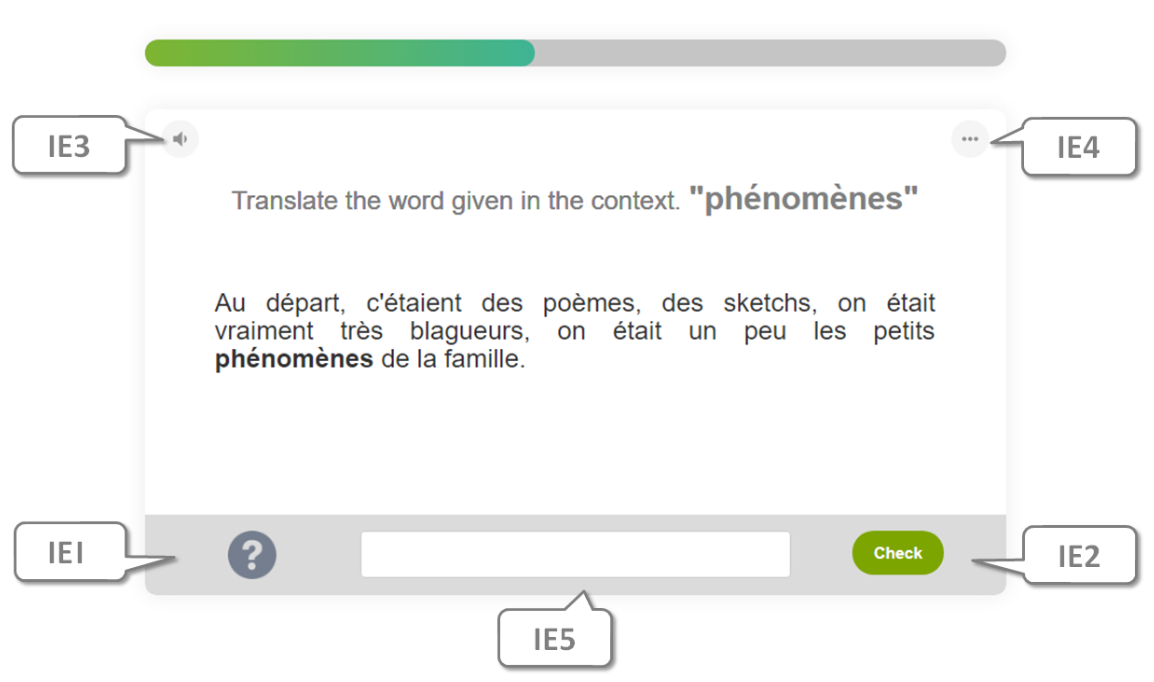
\includegraphics[width=0.9\columnwidth]{figures/exercise_translate}
  \caption{One of the exercise types with which the user is presented asks the user to translate a word in a context that is retrieved from the user's past readings}{
  \label{exercise_translate}
  }
\end{figure}

\ml{The system currently implements three other types of vocabulary practice exercises: one similar to the one in figure, but where the user has to select one of three possible translations, one where the user has to translate to the learned language, not to his known language. A third type of exericse asks the learner to match translations to originals}.

\subsubsection{Selecting Words to Study}

Since a learner might encounter many words that are not understood, we need to prioritize those that are to be studied in exercises. We use three aspects to prioritize words: 

% The words good for study are the ones that are either starred by the user, or are important and of quality based on a set of heuristics. 

\begin{description}

  \item [Important Words] are the ones which appear frequently in the language. For word frequencies we use frequencies computed based on movie subtitles which have been shown to be highly representative to frequencies in human interacitons \cite{New07-subtitles}. 
  
  \item [Quality Context] we favor words that come with a context which is not too short but not too long. 

\end{description}

\subsection{Study Recommender}

The scheduling algorithm is based on an adaptive, response-time-based scheduling algorithm [was developed] to increase the efficiency of perceptual learning by Mettler et al. \cite{Mettler14-ARTS}. After evaluating several alternative scheduling strategies we settled on the Mettler one since it has been proven to have gains with both familiar, seen items as well as with new, unseen instances and the benefits of adaptive scheduling were present at an immediate test as well as at a delay \cite{Mettler14-ARTS}.
